% Copyright 2009 by Tomasz Mazur
% This file may be distributed and/or modified in all ways.

%\documentclass[xcolor=pdftex,t,11pt,handout]{beamer}
\documentclass[xcolor=pdftex,t,11pt]{beamer}

%%%%%%%%%%%%%%%%%%%%%%%%%%%%%%%%%%
%       SET OPTIONS BELOW        %
%%%%%%%%%%%%%%%%%%%%%%%%%%%%%%%%%%
\usepackage[icelandic, english]{babel}
\usepackage{t1enc} 
\usepackage{textcomp}
\usepackage[
% Toggle showing page counter
pagecounter=true,
%
% String to be used between the current page and the
% total page count, e.g. of, /, from, etc.
pageofpages=of,
%
% Defines the shape of bullet points. Available options: circle, square
bullet=circle,
%
% Show a line below the frame title. 
titleline=true,
%
% Set the style of the title page (true for fancy, false for standard)
alternativetitlepage=true,
%
% Institution logo for fancy title page.
titlepagelogo=presentation/beamer/hilogo,
ordinarypageslogo=presentation/beamer/hilogo,
]{presentation/beamer/beamerthemeBerkeley} 

% Select color theme. Available options are:
% mininmal, greenandblue, blue, red
\usepackage{presentation/beamer/beamercolorthemehi}

%Select different font themes.Available options are:
% default, serif, structurebold, structureitalicserif, structuresmallcapsserif
\usefonttheme{structurebold}

\setbeamercovered{transparent}

\newcommand{\bi}{\begin{enumerate}[label={{$\star$}}]\item }
\newcommand{\ei}{\end{enumerate}}

%\renewcommand{\rho}{\varrho}
\renewcommand{\vec}[1]{\mathbf{#1}}
\newcommand{\vphi}{{\mathbf{\phi}}}
\newcommand{\vchi}{{\mathbf{\chi}}}
\newcommand{\vsigma}{{\mathbf{\sigma}}}
\newcommand{\mat}[1]{\mathbf{#1}}
\newcommand{\R}{{\mathbb R}}
\newcommand{\Exp}[1]{{\mathbb E}\left[#1\right]}
\newcommand{\Prob}[1]{{\mathcal P}\left(#1\right)}
\newcommand{\strng}[1]{{\mbox{\tt #1}}}
\newcommand{\inner}[2]{\big<{#1}\cdot{#2}\big>}
\newcommand{\abs}[1]{\lvert#1\rvert}
\newcommand{\norm}[1]{\lVert#1\rVert}
\newcommand{\argmax}{\mathop{\rm argmax}}
\newcommand{\argmin}{\mathop{\rm argmin}}
\newcommand{\nchoosek}[2]{\tiny \left(\begin{array}{c}#1\\#2\end{array}\right)}
\newcommand{\condset}[2]{\left\{#1\;\middle|\;#2\right\}}
\newcommand{\limit}[3]{\lim_{#2}#1=#3}
\newcommand{\bigOh}[1]{{O}\left(#1\right)}

% percentage relative deviation from optimality
\newcommand{\Namerho}{Deviation from optimality, $\rho$}
\newcommand{\namerho}{deviation from optimality, $\rho$}
\newcommand{\fullnamerho}{\namerho, defined by~\cref{eq:rho}}
\newcommand{\Problem}[2][ ]{$\mathcal{P}_{#2}^{#1}$}
\newcommand{\jrnd}[2]{\Problem[#1 \times #2]{j.rnd}}
\newcommand{\jrndJ}[2]{\Problem[#1 \times #2]{j.rnd,J_1}}
\newcommand{\jrndM}[2]{\Problem[#1 \times #2]{j.rnd,M_1}}
\newcommand{\jrndn}[2]{\Problem[#1 \times #2]{j.rndn}}
\newcommand{\frnd}[2]{\Problem[#1 \times #2]{f.rnd}}
\newcommand{\frndn}[2]{\Problem[#1 \times #2]{f.rndn}}
\newcommand{\fjc}[2]{\Problem[#1 \times #2]{f.jc}}
\newcommand{\fmc}[2]{\Problem[#1 \times #2]{f.mc}}
\newcommand{\fmxc}[2]{\Problem[#1 \times #2]{f.mxc}}

\newcommand{\dr}{dispatching rule}
\newcommand{\cdr}{composite priority \dr}
\newcommand{\sdr}{single priority \dr}
\newcommand{\Fsp}{Flow-shop}
\newcommand{\Jsp}{Job-shop}
\newcommand{\fsp}{flow-shop}
\newcommand{\jsp}{job-shop}
\newcommand{\FSP}{FSP}
\newcommand{\JSP}{JSP}
\newcommand{\Jrnd}{\JSP~random}
\newcommand{\JrndJ}{\JSP~random with job variation}
\newcommand{\JrndM}{\JSP~random with machine variation}
\newcommand{\Jrndn}{\JSP~random-narrow}
\newcommand{\Frnd}{\FSP~random}
\newcommand{\Frndn}{\FSP~random narrow}
\newcommand{\Fjc}{\FSP~job-correlated}
\newcommand{\Fmc}{\FSP~machine-correlated}
\newcommand{\Fmxc}{\FSP~mixed-correlated}

% job-related
\newcommand{\phiproc}{$\phi_1$}
\newcommand{\phistartTime}{$\phi_2$}
\newcommand{\phiendTime}{$\phi_3$}
\newcommand{\phiarrivalTime}{$\phi_4$}
\newcommand{\phiwait}{$\phi_5$}
\newcommand{\phijobTotProcTime}{$\phi_6$}
\newcommand{\phijobWrm}{$\phi_7$}
\newcommand{\phijobOps}{$\phi_8$}
\newcommand{\phiJobRelated}{\phiproc\!-\phijobOps}
% mac-related
\newcommand{\phimacFree}{$\phi_{9}$}
\newcommand{\phimacTotProcTime}{$\phi_{10}$}
\newcommand{\phimacWrm}{$\phi_{11}$}
\newcommand{\phimacOps}{$\phi_{12}$}
\newcommand{\phireducedSlack}{$\phi_{13}$} 
\newcommand{\phimacSlack}{$\phi_{14}$}
\newcommand{\phiallSlack}{$\phi_{15}$}
\newcommand{\phiSlackRelated}{\phireducedSlack\!-\phiallSlack}
\newcommand{\phimakespan}{$\phi_{16}$}
\newcommand{\phiMacRelated}{\phimacFree\!-\phimakespan}
% global
\newcommand{\phiSPT}{$\phi_{17}$}
\newcommand{\phiLPT}{$\phi_{18}$}
\newcommand{\phiLWR}{$\phi_{19}$}
\newcommand{\phiMWR}{$\phi_{20}$}
\newcommand{\phiSDRRelated}{\phiSPT\!-\phiMWR}
\newcommand{\phiRND}{\phi_{\text{RND}}}
\newcommand{\phiRNDmean}{$\phi_{21}$}
\newcommand{\phiRNDstd}{$\phi_{22}$}
\newcommand{\phiRNDmin}{$\phi_{23}$}
\newcommand{\phiRNDmax}{$\phi_{24}$}
\newcommand{\phiRNDRelated}{\phiRNDmean\!-\phiRNDmax}
\newcommand{\phiGlobalRelated}{\phiMWR\!-\phiRNDmax}
\newcommand{\phiLocalRelated}{\phiproc\!-\phimakespan}
% feature count
\newcommand{\NrFeatLocal}{16}
\newcommand{\NrFeatGlobal}{4}
\newcommand{\NrFeatTotal}{24}

\hyphenpenalty=800
\hbadness=2500

\hyphenation{heur-ist-ics}
\hyphenation{algo-rithm}

\usepackage{amsmath,amssymb}

\usepackage{tabularx}
\usepackage{multirow}
\usepackage{rotating}
\newcommand{\rot}[1]{\begin{sideways}#1\end{sideways}}

\usepackage[inline]{enumitem}
\setlist[enumerate,1]{
    label=\textit{\roman*)},
    before=\unskip{: }, 
    itemjoin={{; }}, itemjoin*={{, and }},
    after={{. }}
    }

\usepackage{booktabs} % \toprule \midrule \bottomrule

\usepackage{comment}

%\usepackage[retainorgcmds]{IEEEtrantools}

\usepackage{aliascnt}
\usepackage[capitalise,nameinlink]{cleveref} % must come last! 
% provide singular and plural names of the categories "paper"
\crefname{paper}{Paper}{Papers}
\Crefname{paper}{Paper}{Papers}

% Nomenclature
\usepackage{nomencl}
\makenomenclature
\renewcommand\nomgroup[1]{
  \ifthenelse{\equal{#1}{F}}{\item[\textbf{Rice's Framework}]}{
    \ifthenelse{\equal{#1}{J}}{\item[\textbf{\Jsp\ Scheduling}]}{ 
      \ifthenelse{\equal{#1}{O}}{\item[\textbf{Ordinal Regression}]}{ 
        \ifthenelse{\equal{#1}{S}}{\item[\textbf{Surrogate Modelling}]}{ 
          \ifthenelse{\equal{#1}{X}}{\item[\textbf{Experimental Settings}]}{ 
            \ifthenelse{\equal{#1}{Y}}{\item[\textbf{Subscripts and 
                Superscripts}]}{
              \ifthenelse{\equal{#1}{Z}}{\item[\textbf{Acronyms}]}{ 
              }
            }
          }
        }
      }
    }
  }
}
\usepackage{xifthen}

\usepackage{algorithm}
\usepackage{algpseudocode}
\makeatletter
\def\BState{\State\hskip-\ALG@thistlm}
\makeatother
\algnewcommand\algorithmicto{~\textbf{to}~}
\algnewcommand\algorithmicand{~\textbf{and}~}
\algrenewtext{For}[3]%
{\algorithmicfor\ $#1 \gets #2 \algorithmicto\ #3$~\algorithmicdo}
\usepackage{ifthen}
\usepackage{float}
\usepackage{morefloats}

%\usepackage{footnote}
%\usepackage[bottom,perpage,symbol*]{scripts/footmisc}

\newcommand{\tcr}[1]{{\color{red} #1}}
\newcommand{\tcb}[1]{{\color{blue} #1}}
\newcommand{\tcg}[1]{{\color{green} #1}}
\newcommand{\Alice}{Alice}
\newcommand{\fullnameAlice}{Adaptive Learning Intelligent Composite rulEs}

\usepackage[retainorgcmds]{packages/IEEEtrantools}

%\usetikzlibrary{angles} % gametree

\setlist[description]{leftmargin=1cm,labelindent=1cm} % put your own shorthand declarations here
\usepackage{longtable}
\usepackage{tabularx}
\usepackage{multirow}
\usepackage{rotating}
\newcommand{\rot}[1]{\begin{sideways}#1\end{sideways}}


\setlist[description]{leftmargin=1cm,labelindent=1cm}
\usepackage[retainorgcmds]{packages/IEEEtrantools}
\usepackage{nicefrac}
\usepackage{booktabs} % \toprule \midrule \bottomrule

\usepackage{comment}
\usepackage[splitrule,bottom,perpage,symbol*]{packages/footmisc}
\setfnsymbol{wiley} % wiley: ∗, ∗∗, †, ‡, §, ¶, ||.
\renewcommand{\mpfootnoterule}{}
\let\splitfootnoterule\footnoterule
\renewcommand{\thempfootnote}{\fnsymbol{mpfootnote}}

\usepackage{aliascnt}
\usepackage[capitalise,nameinlink]{cleveref} % must come last! 
% provide singular and plural names of the categories "paper"
\crefname{paper}{Paper}{Papers}
\Crefname{paper}{Paper}{Papers}
\crefname{ineq}{Ineq.}{Ineqs.}
\Crefname{ineq}{Inequality}{Inequalities}
\creflabelformat{ineq}{~\upshape(#2#1#3)}

\usepackage{soul} % strikeout text \st{text}
%\setstcolor{gray}

\usepackage{algorithm}
\usepackage{algpseudocode}
\makeatletter
\def\BState{\State\hskip-\ALG@thistlm}
\makeatother
\algnewcommand\algorithmicto{~\textbf{to}~}
\algnewcommand\algorithmicand{~\textbf{and}~}
\algrenewtext{For}[3]%
{\algorithmicfor\ $#1 \gets #2 \text{\algorithmicto} #3$~\algorithmicdo}

\newcommand{\ntodo}[2][]{\todo[#1]{\thesection{}. #2}}
\newcommand{\todoFind}[1]{\ntodo[color=red]{#1}}
\newcommand{\todoExtend}[1]{\ntodo[color=blue]{#1}}
\newcommand{\todoPapers}[1]{\ntodo[color=green]{#1}}
\newcommand{\todoWrite}[1]{\ntodo[inline,color=yellow]{#1}}

\usepackage{packages/forest} % for figures/orlib-methods
\tikzstyle{arrow} = [->,>={latex}, draw=black]

% ------------------------------------------------------- for alice.tex
\usepackage{etoolbox}
\newcommand\chquote[3][]{%
    \ifstrempty{#1}{%
        \emph{#3} 
    }{%
    #1: \emph{\st{#3}} 
}%
\hfill \textbf{#2}\\\\
}
 % put your own shorthand declarations here

\graphicspath{{presentation/},{figures/}}
\DeclareGraphicsExtensions{.eps,.png}
%%%%%%%%%%%%%%%%%%%%%%%%%%%%%%%%%%
%       PRESENTATION INFO        %
%%%%%%%%%%%%%%%%%%%%%%%%%%%%%%%%%%
\author[Helga]{Helga Ingimundard\'{o}ttir}
\title{\Alice}
\subtitle{\fullnameAlice}
\institute{University of Iceland}	
\date{June 30, 2016}

\newcommand<>{\tikzMe}[1]{% previously: \def\tikzMe<#1>#2{…
    \tikz[baseline]\node[BeamerAlert=#2,anchor=base] {#1};
}

\begin{document}

%%%%%%%%%%%%%%%%%%%%%%%%%%%%%%%%%%
%       SLIDE DEFINITIONS        %
%%%%%%%%%%%%%%%%%%%%%%%%%%%%%%%%%%

\begin{frame}
	\titlepage
\end{frame}

\section{Introduction}
\frame{
\frametitle{Introduction}
Motivation
\bi The general goal is to train optimisation algorithms, for an 
arbitrary problem domain, using data\ei
Contribution
\bi The main contribution of this thesis is towards a better understanding of 
how this training data should be constructed\ei 
}
\frame[label=alice]{
    \frametitle{Framework for Algorithm Learning}
    \setbeamercovered{invisible}
\begin{figure}[t]\centering
\tikzset{
    block/.style = {draw, fill=gray!10, rectangle, text width=7em, 
        align=center,font=\bfseries\sffamily},
    txt/.style = {font=\small\sffamily,text width=9em,align=center,midway},
    ltxt/.style = {txt,left,align=right},
    rtxt/.style = {txt,right,align=left},
    rice/.style = {fill=gray!35},    
    invisible/.style={opacity=0,text opacity=0},
    visible on/.style={alt=#1{}{invisible}},
    alt/.code args={<#1>#2#3}{%
        \alt<#1>{\pgfkeysalso{#2}}{\pgfkeysalso{#3}} 
    },
    beameralert/.style={alt=<#1>{fill=red!30}{},anchor=base},
    BeamerAlert/.style={alt=#1{fill=red!30,rounded corners}{},anchor=base}
}
\vspace{-12pt}
\resizebox{\columnwidth}{!}{%
% The block diagram code is probably more verbose than necessary
\begin{tikzpicture}[auto, node distance=2.3cm]%,>=latex']
\node [block, rice, beameralert=1] (P) {Problem space $\vec{z}\in\mathcal{P}$};
\node [block, beameralert=2, below of=P] (I) {Subspace of instances 
\mbox{$\vec{x}\in \mathcal{P}' \subset \mathcal{P}$}};
\node [block, rice, beameralert=3, below of=I] (Phi) {Feature space 
$\vphi(\vec{x})\in\Phi\subset\mathcal{F}$};
\node [block, beameralert=6, right of=P, xshift=3.4cm] (F) 
{Footprints in instance space};
\node [block, rice, beameralert=5, right of=I, xshift=3.4cm] (Y) 
{Performance space $y\in\mathcal{Y}$};
\node [block, rice, beameralert=4, right of=Phi, xshift=3.4cm] (A) 
{Algorithm space $a\in\mathcal{A}$};

\draw [arrow] (P) -- node[ltxt] {instance selection} (I);
\draw [arrow] (I) -- node[ltxt] {feature selection $\vphi$} (Phi);
\draw [arrow] (Phi) -- (A);
\draw [arrow] (A) -- node[rtxt] {$\Upsilon(a,\vphi(\vec{x}))$ apply alg. $a$ to 
    instance $\vec{x}$} (Y);
\draw [arrow] (Y) -- node[rtxt] {define algorithm footprint 
    $f(y(a,\vec{x}))$} (F);
\draw [arrow] (F) -- node[txt] {infer algorithm performance on all 
    $\vec{z}\in\mathcal{P}$} (P);

\visible<7->{
\node [block, beameralert=7, below of=Phi] (Psi) {Preference set $\Psi \subset 
\Phi$};
\node [block, beameralert=8, right of=Psi, xshift=3.4cm] (PREF) {Preference 
learning};
\draw [arrow,dotted] (Phi) -- node[ltxt] {sample preference pairs} (Psi);
\draw [arrow,dotted] (Psi) -- (PREF);
\draw [arrow,dotted] (PREF) -- node[rtxt] {train algorithm $a$} (A);
}
\visible<9>{
    \draw [arrow,dotted] (F) -- node[txt,sloped,above] {feature feedback} (Psi);
}
\end{tikzpicture}}
\end{figure}
}

\section{Problem space}\againframe<1>{alice}

\frame{
    \frametitle{Job Shop Scheduling (\JSP)}
    Simple \jsp\ is where $n$ jobs are scheduled on 
    a set of $m$ machines, subject to constraints  
    \bi each job must follow a predefined machine order,  
    \item that a machine can handle at most one job at a time\ei  
    \textbf{Objective:} schedule the jobs so as to minimise the maximum 
    completion time, i.e., makespan, $C_{\max}$.
}
\frame{\frametitle{Dispatching rules}
    Dispatching rules (DR) are consecutive executions found by
    \bi Starting with an empty schedule and adding on one operation at a time. 
    \item When a machine is free the DR inspects the available jobs and 
    selects the one with the \alert{highest priority}. 
    \item Complete schedule consists of $\ell=n\cdot m$ sequential dispatches.
    \item At each dispatch $k$, \alert{features} $\vphi(k)$ for the temporal 
    schedule are calculated\ei
}

\frame{
    \frametitle{Mad Hatter tea-party (definition)}
    \begin{columns}
        \begin{column}{0.35\columnwidth}
            The attending guests
            \bii{$J_\arabic*$)} Alice\label{guest:alice}
                \item March Hare\label{guest:marchhare}
                \item Dormouse\label{guest:dormouse}
                \item Mad Hatter\label{guest:madhatter}\ei
        \end{column}
        \begin{column}{0.65\columnwidth}
            They all have to
            \bii{$M_\arabic*$)} have wine or pour tea
                \item spread butter
                \item get a haircut
                \item check the time of the broken watch
                \item say what they mean\ei
        \end{column}
    \end{columns}
    \vspace{6pt}
    This can be considered as is a typical $4\times5$ \jsp, where
    \bi our guests are the jobs
    \item their tasks are the machines
    \item objective is to minimise $C_{\max}$ (when Alice can leave)\ei
}
\frame{
    \frametitle{Mad Hatter tea-party (action states)}    
    \tikzstyle{vertex}=[circle,fill=black!15,minimum size=20pt,inner sep=0pt]
\tikzstyle{completed vertex} = [vertex, fill=red!24]
\tikzstyle{possible vertex} = [vertex, fill=black!25]
\tikzstyle{edge} = [draw,thick,->,black!20]
\tikzstyle{proc} = [font=\small, below]
\tikzstyle{completed edge} = [draw,line width=2pt,->,red!50]
\tikzstyle{possible edge} = [draw,line width=4pt,->,black!20]
\tikzstyle{job line} = [line width=4mm,join=round]
\usetikzlibrary{backgrounds}

    \setbeamercovered{transparent}
    \begin{columns}
    \begin{column}[T]{0.5\columnwidth}
    \uncover<1>{\resizebox{\columnwidth}{!}{\input{figures/example.graph.k0.tex}}}
    \\\vspace{24pt}
    \uncover<2>{\resizebox{\columnwidth}{!}{\pgfdeclarelayer{bgk20}
\pgfsetlayers{bgk20,main}  
\begin{tikzpicture}[scale=1.3, auto, swap]
    % Draw the network
    % First we draw the jobs
    \node at (-1,0) [fill=set1red] {$J_1$};
    \node at (-1,1) [fill=set1blue] {$J_2$};
    \node at (-1,2) [fill=set1green] {$J_3$};
    \node at (-1,3) [fill=set1purple] {$J_4$};
    % Second draw the machines / vertices
    \foreach \pos/\name/\mac/\proc in {{(0,1.5)/Source},{(6,1.5)/Sink},
        {(1,0)/J1M1/M_1/26},{(2,0)/J1M2/M_2/25},{(3,0)/J1M3/M_3/40},{(4,0)/J1M4/M_4/15},{(5,0)/J1M5/M_5/42},
        {(1,1)/J2M1/M_1/18},{(2,1)/J2M2/M_2/86},{(3,1)/J2M3/M_3/86},{(4,1)/J2M4/M_4/68},{(5,1)/J2M5/M_5/84},
        {(1,2)/J3M1/M_1/20},{(2,2)/J3M3/M_3/23},{(3,2)/J3M2/M_2/59},{(4,2)/J3M4/M_4/33},{(5,2)/J3M5/M_5/96},
        {(1,3)/J4M4/M_4/13},{(2,3)/J4M3/M_3/55},{(3,3)/J4M1/M_1/40},{(4,3)/J4M5/M_5/99},{(5,3)/J4M2/M_2/47}}
    \node[completed vertex] (\name) at \pos {$\mac$};
    % Selected trajectory
    \path[completed edge] (J4M4) to[bend right] (J2M1);
    \path[completed edge] (J1M5) to[bend left=17] (J4M3);
    \foreach \source/ \dest in {
        Source/J4M4, J2M1/J3M1, J3M1/J3M3, J3M3/J1M1, J1M1/J1M2, J1M2/J1M3, 
        J1M3/J1M4, J1M4/J1M5, J4M3/J4M1, J4M1/J3M2, J3M2/J3M4, J3M4/J2M2, 
        J2M2/J2M3, J2M3/J2M4, J2M4/J2M5, J2M5/J3M5, J3M5/J4M5, J4M5/J4M2, 
        J4M2/Sink} 
    \path[completed edge] (\source) -- (\dest);
    % draw background for job's swimlane
    \begin{pgfonlayer}{bgk20}
    \filldraw [job line,set1red!10]
    (J1M1.north -| J1M1.west) rectangle (J1M5.south -| J1M5.east);
    \filldraw [job line,set1blue!10]
    (J2M1.north -| J2M1.west) rectangle (J2M5.south -| J2M5.east);
    \filldraw [job line,set1green!10]
    (J3M1.north -| J3M1.west) rectangle (J3M5.south -| J3M5.east);
    \filldraw [job line,set1purple!10]
    (J4M4.north -| J4M4.west) rectangle (J4M2.south -| J4M2.east);
    \end{pgfonlayer}
    \end{tikzpicture}
    }}
    \end{column}
    \begin{column}[T]{0.5\columnwidth}
    \only<1-2>{\resizebox{\columnwidth}{!}{  \begin{tikzpicture}
  \node[anchor=south west,inner sep=0] (image) at (0,0,0) 
  {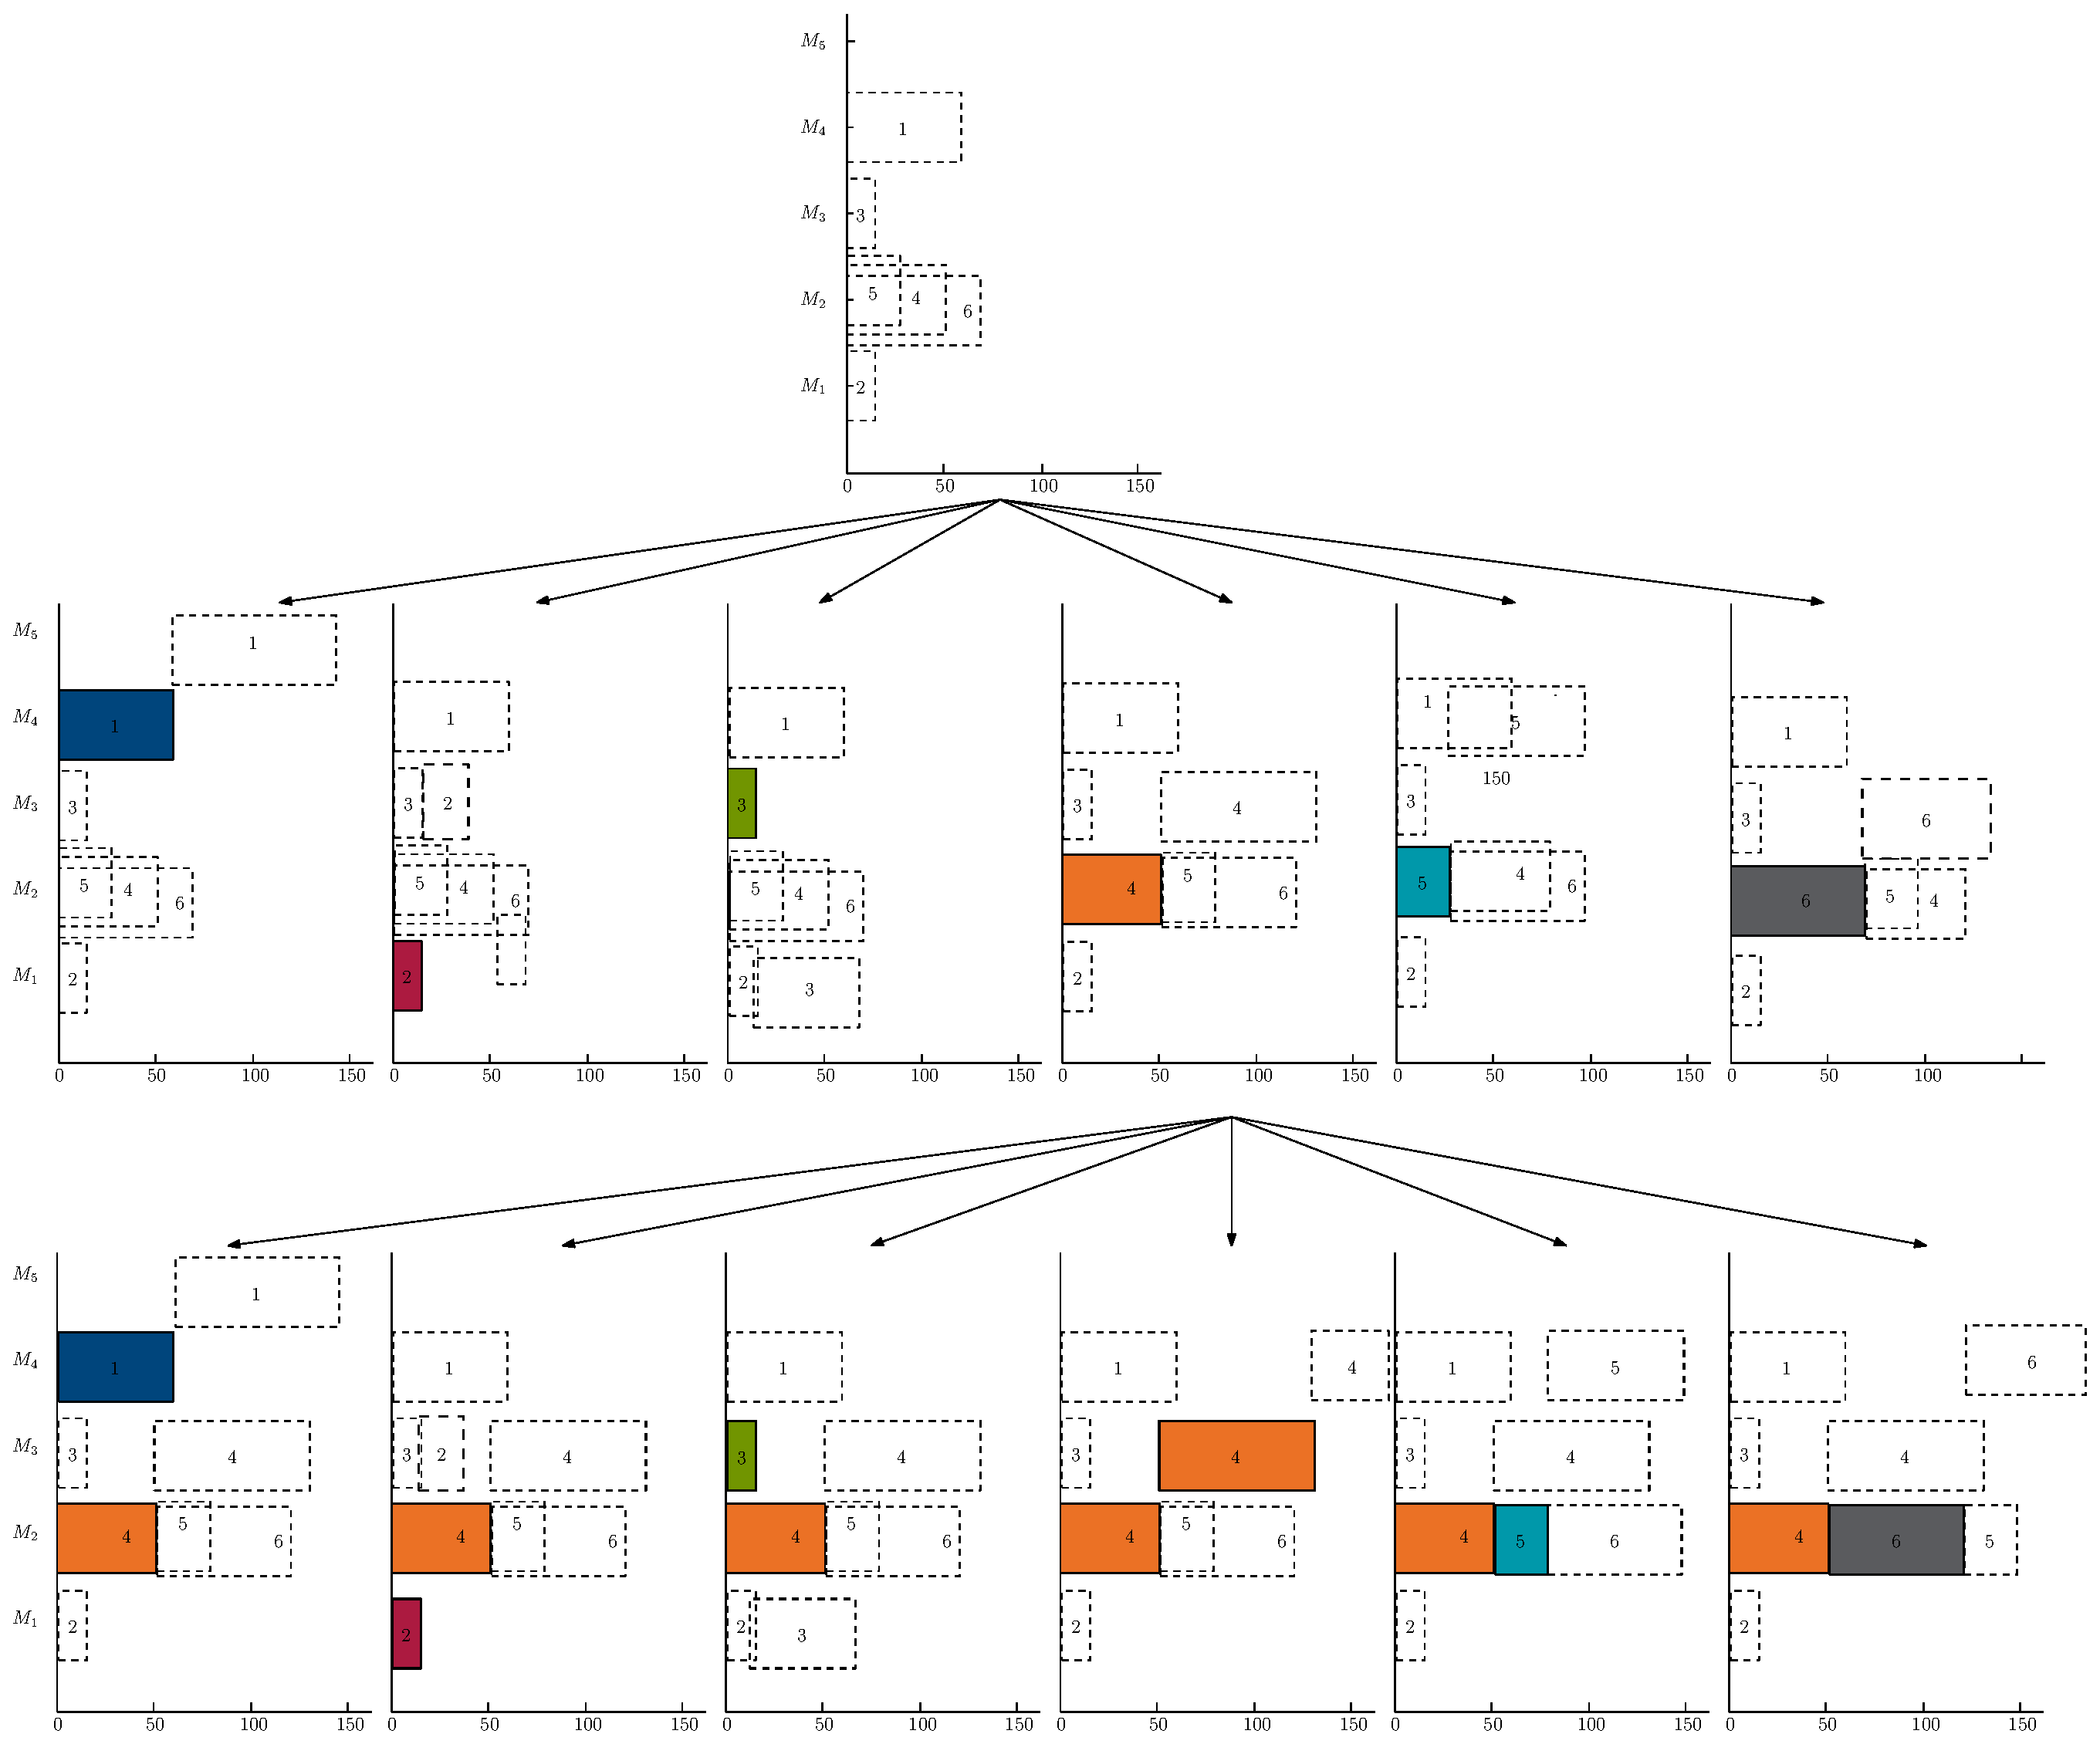
\includegraphics[width=\textwidth]{gametree}};
  \begin{scope}[x={(image.south east)},y={(image.north west)}]
  %% next four lines will help you to locate the point needed by forming a 
  %%grid. comment these four lines in the final picture.↓
  %\draw[help lines,xstep=.1,ystep=.1] (0,0) grid (1,1);
  %\draw[help lines,xstep=.05,ystep=.05] (0,0) grid (1,1);
  %\foreach \x in {0,1,...,9} { \node [anchor=north] at (\x/10,0) {0.\x}; }
  %\foreach \y in {0,1,...,9} { \node [anchor=east] at (0,\y/10) {0.\y};}
  %% upto here↑
  \node (J0) at (0.5,0.71) {};
  \node (J1) at (0.19,0.65) {};
  \node (J2) at (0.42,0.65) {};
  \node (J3) at (0.65,0.65) {};
  \node (J4) at (0.85,0.65) {};
  \draw[-latex] (J0) to[out=-20,in=+20] (J1);
  \draw[-latex] (J0) to[out=-20,in=+20] (J2);
  \draw[-latex] (J0) to[out=-20,in=+20] (J3);
  \draw[-latex] (J0) to[out=-20,in=+20] (J4);
  \node (J4) at (0.82,0.38) {};
  \node (J4J1) at (0.19,0.31) {};
  \node (J4J2) at (0.42,0.31) {};
  \node (J4J3) at (0.65,0.31) {};
  \node (J4J4) at (0.85,0.31) {};
  \draw[-latex] (J4) to[out=-20,in=+20] (J4J1);
  \draw[-latex] (J4) to[out=-20,in=+20] (J4J2);
  \draw[-latex] (J4) to[out=-20,in=+20] (J4J3);
  \draw[-latex] (J4) to[out=-20,in=+20] (J4J4);
  \end{scope}
  \end{tikzpicture}
}}
    \visible<3>{\resizebox{\columnwidth}{!}{\input{figures/example.graph.k10.tex}}}
    \\\vspace{24pt}
    \includegraphics<3>[width=\columnwidth]{figures/{example.gantt}.pdf}
    \end{column}
    \end{columns}
}
\frame{
    \frametitle{Mad Hatter tea-party (SDRs)}
    \includegraphics[width=\columnwidth,height=.9\textheight]{figures/{example.gantt.SDRs}.pdf}
}
\section{Subspace of instances}\againframe<2>{alice}

\section{Feature space}\againframe<3>{alice}
\frame{\frametitle{Features for \JSP}\label{tbl:features}
    \begin{table}[t!] \centering
    \vspace{-14pt}
    \resizebox{\textheight}{!}
    {\scriptsize 
    \renewcommand{\arraystretch}{0.6}
    \begin{tabular}{ccl}
        \toprule
        %& $\vphi$ & Feature description \\  \midrule
        \multirow{10}{*}{\rot{\textbf{job}}}
        & $\phiproc$ & job processing time \\
        & $\phistartTime$ & job start-time \\
        & $\phiendTime$ & job end-time \\
        & $\phiarrivalTime$ & job arrival time \\ 
        & $\phiwait$ & time job had to wait \\ 
        & $\phijobTotProcTime$ & total processing time for job \\
        & $\phijobWrm$ & total work remaining for job \\
        & $\phijobOps$ & number of assigned operations for job \\ 
        \midrule
        \multirow{10}{*}{\rot{\textbf{machine}}}
        & $\phimacFree$ & when machine is next free \\
        & $\phimacTotProcTime$ & total processing time for machine \\
        & $\phimacWrm$ & total work remaining for machine \\
        & $\phimacOps$ & number of assigned operations for machine \\
        & $\phireducedSlack$ & change in idle time by assignment \\
        & $\phimacSlack$ & total idle time for machine \\
        & $\phiallSlack$ & total idle time for all machines \\
        & $\phimakespan$ & current makespan \\
        \midrule
        \multirow{12}{*}{\rot{\textbf{final makespan}}}
        & $\phiSPT$ & final makespan using SPT \\
        & $\phiLPT$ & final makespan using LPT \\
        & $\phiLWR$ & final makespan using LWR \\
        & $\phiMWR$ & final makespan using MWR \\
        & $\phiRND$ & final makespans using 100 random rollouts \\ 
        & $\phiRNDmean$ & mean for $\phiRND$ \\ 
        & $\phiRNDstd$ & standard deviation for $\phiRND$ \\
        & $\phiRNDmin$ & minimum value for $\phiRND$\\ 
        & $\phiRNDmax$ & maximum value for $\phiRND$\\ 
        \bottomrule
    \end{tabular}
    }
    \end{table}
}

\section{Algorithm Space}\againframe<14|handout:0>{alice}
\frame[label=algorithms]{
    \frametitle{Various Methods for Solving \JSP}\framesubtitle{Based on 
    Jain and Meeran (1999)}
    %http://tex.stackexchange.com/questions/244742/work-breakdown-structure-wbs-horizontally
\usetikzlibrary{shapes,positioning,shadows,trees,fit,arrows,calc}

\tikzset{
        %every node/.style={inner sep=1,outer sep=1},
        txtLrg/.style={rectangle, draw, %text width=2cm, 
          align=flush center, 
          font=\bfseries\scriptsize\sffamily, thin},
        txtSml/.style  = {txtLrg, align=left, font=\tiny\sffamily},
        txtComment/.style = {font=\tiny\sffamily, xshift=-0.4cm, near start,
            text width=5cm, rotate=90, align=left},
        txtRef/.style= {}, %font=\tiny\sffamily, midway, above, sloped},
        hybrid/.style = {}, %-,draw=black, dashed},
        based/.style = {arrow, dotted},
        long/.style = {minimum width=7em},
        medium/.style = {minimum width=6em},
        small/.style = {minimum width=5em},
        verysmall/.style = {minimum width=2.7em}
}

\forestset{
    normal/.style  = {for tree={child anchor=west, parent anchor=east}},
    rotated/.style = {for tree={child anchor=north, parent anchor=south},
        rotate=90},
    unrotate/.style = {normal, rotate=-90},
    root/.style  = {txtLrg, rotated, fill=gray!50},
    onode/.style = {txtLrg, rotated, fill=gray!25},
    tnode/.style = {txtSml, normal, fill=gray!10},
    thesis/.style = {fill=red!50},
    alert/.style = {draw=red,thick},
    emphasis/.style = {tikz={
            \node<2>[fill,fill opacity=.1,purple,thick,fit to tree]{};}},
    edge from parent/.style={arrow, edge from parent fork right}
}

\rot{\rot{\rot{\resizebox{.95\textheight}{!}{%
\begin{forest}
for tree={
    s sep=3pt, % distance between siblings
    grow=east,
    growth parent anchor=east,
    edge path={\noexpand\path[\forestoption{edge},->, >={latex}] 
        (!u.parent anchor) -- +(5pt,0pt) |- (.child anchor)
        \forestoption{edge label};}
}
[\JSP, root
    [Approximation, root, edge label = {node[txtComment, left]{
            Approximations methods, or heuristics, are generally time 
            efficient, but do not necessarily attain the global optimum.}},
        [General algorithms\\(iterative methods), onode, 
            [Artificial intelligence, onode
                [Machine\\learning, onode,  
                    [Roll-out / Pilot method, tnode, long, thesis]
                    [Reinforcement learning, tnode, long]
                    [Decision tree, tnode, long]
                    [Imitation\\learning, onode, emphasis, thesis, 
                    name=IL
                        [Active, onode, 
                            [DAgger, tnode, small, name=DAgger]
                        ]
                        [Passive, onode, 
                            [Follow the expert, tnode, small]
                            [Perturbed leader, tnode, small]
                            [Follow heuristics, tnode, small]
                        ]
                    ]
                ]
                [Constraint satisfaction,tnode, long]
%                [Expert systems,tnode, medium]
                [Ant colony optimisation,tnode, long, name=ACO]
                [Artificial neural network,tnode, long, name=ANN]
            ]
            [Local search, onode
                [Reinsertion algorithms, tnode, long]
                [Threshold alg., onode, long, unrotate
                    [Simulated annealing, tnode, medium, name=SA]
                    [Threshold accepting, tnode, medium
                    ]
                    [Iterative development, tnode, medium]
                ]
                [Large step optimisation, tnode, long]
                [Tabu Search, tnode, long, name=TS]
                [Evolutionary computation,tnode, long, thesis, 
                    [Genetic local search, tnode, medium]
                ]
                [Genetic algorithms, tnode, long, name=GA
                    [Genetic programming, tnode, medium, name=GP]
                ]
                [Variable depth search, tnode, long, name=VDS]
            ]
        ]
        [Tailored algorithms\\(constructive methods), onode
            [Bottleneck based\\heuristics, onode, unrotate
                [Shifting bottle-\\neck procedure, tnode, name=SBP
                    [Beam search, tnode, name=BS]
                ]
            ]
            %[Insertion algorithm, tnode]
            [Priority DR, onode, emphasis, thesis,  
                [SDR, onode
                    [SPT, tnode, verysmall]
                    [LPT, tnode, verysmall]
                    [LWR, tnode, verysmall]
                    [MWR, tnode, verysmall]
                ]
                [CDR, tnode, name=CDR, rotated]
            ] 
         ]
    ]
    [Optimisation, root, edge label = {node[txtComment, right]{
            Exact methods guarantee an optimal solution, although for NP-hard 
            problems they are intractable for high dimensionality.}},
        [Efficient methods, tnode] 
        [Enumerative methods, onode, 
            [Branch \& Bound, tnode, name=BB, thesis]
            [Mathematical, onode
                [Surrogate duality, tnode, long] 
                [Lagrangian relaxation, tnode, long] 
                [Decomposition methods, tnode, long] 
                [Integer linear programming, tnode, long] 
                [Mixed integer lin.prog., tnode, long] 
            ]
        ]
    ]
]
\draw[arrow] (ANN) -| (SA);
\draw[arrow] (VDS) -| (SBP);
\draw<2>[arrow,alert] (IL.east) to[out=90,in=30] (CDR.east);
\pause
\end{forest}
}}}}
}

\section{Performance space}\againframe<5>{alice}
\section{Footprints in instance space}\againframe<6>{alice}
\section{Preference set}\againframe<7>{alice}
\section{Preference learning}\againframe<8>{alice}
\frame{\frametitle{Ordinal Regression}
    Preference learning
    \bi Mapping of points to ranks: $ \{h(\cdot) : \Phi \mapsto Y\}$ where 
    $$\vphi_o \succ \vphi_s \quad \iff \quad h(\vphi_o) > h(\vphi_s)$$
    \item The preference is defined by a linear function:
    $$ h(\vphi) = \sum_{i=1}^d w_i \vphi $$
    based on $d$ features -- optimised w.r.t. $\vec{w}$\ei	
}
\frame{\frametitle{Learning methods}
    Passive imitation learning
        \bi Prediction with expert advice, $\pi_\star$ -- Gurobi\ei
    \pause 
    Active imitation learning
        \bi Follow the perturbed leader (OPT$\epsilon$)
        \pause\item Dataset Aggregation (DAgger)
        $$ \pi_i = \beta_i \pi_\star + (1-\beta_i)\hat{\pi}_{i-1}$$
        where $\hat{\pi}_{i-1}$ is the previous learned model, \pause and 
        $\hat{\pi}_i$ learns on
        $$ \Phi^{\text{DA}i} = \bigcup_{i'=0}^i \Phi^{\text{IL}i'}$$
        aggregated dataset of all previous iterations\ei   
}
\frame{\frametitle{DAgger}
\begin{algorithmic}[1]
\Require $T\geq1$
\Procedure{DAgger}{$\pi_\star,\Phi^{\IL{0}},T$}
    \State $\hat{\pi}_0 \gets$ \Call{Train}{$\Phi^{\IL{0}}$}
        \Comment{initial model, iff $\Phi^{\IL{0}}=\Phi^{\OPT}$}
\pause 
    \For{i}{1}{T} \Comment{at each imitation learning iteration}
\pause 
        \State Let $\pi_i = \beta_i\pi_\star + (1-\beta_i)\hat{\pi}_{i-1}$
\pause 
        \State Sample a $K$-solution using $\pi_i$
            \Comment{\Call{IL}{$i,\hat{\pi}_{i-1},\pi_\star$}}
\pause      
        \State $\Phi^{\IL{i}} = \{(s,\pi_\star(s))\}$ 
            \Comment{visited by $\pi_i$ and actions by $\pi_\star$}
\pause           
        \State $\Phi^{\DA{i}} \gets \Phi^{\DA{i-1}} \cup \Phi^{\IL{i}}$ 
            \Comment{aggregate datasets}
\pause
        \State $\hat{\pi}_{i+1} \gets$ \Call{Train}{$\Phi^{\DA{i}}$}
            \Comment{preference model}
    \EndFor
\pause
    \State \Return best $\hat{\pi}_i$ on validation \Comment{best preference 
    model}
\EndProcedure
\end{algorithmic}
    
}
\frame{\frametitle{\Namerho}
    \includegraphics[width=\columnwidth]{figures/{j.rnd}/{boxplot.summary.10x10}.pdf}
}
\section{Conclusions}\againframe<9>{alice}

\frame{
\frametitle{Thank you for your attention}
\begin{columns}[T]
    \begin{column}{0.5\columnwidth} 
        \vspace{36pt}
        \begin{center}
            Helga Ingimundard\'{o}ttir\\
            \url{hei2@hi.is}
        \end{center}
        \vspace{36pt}
        Supplementary material
        \bi \href{https://tgax89.rhi.hi.is:3838/alice}{Shiny application}
            \item \href{https://github.com/ALICE-InRu/Cheshire}{Github} 
        \ei
    \end{column}
    \begin{column}{0.5\columnwidth}
        \includegraphics[width=\columnwidth]{tenniel/queen-alice.jpg}
    \end{column}    
\end{columns}
}
\end{document}